\section{Indici: Concetti Fondamentali per gli Esercizi}
Un indice è una struttura dati che migliora la velocità di recupero dei dati. Immaginalo come l'indice analitico di un libro.

\subsection{Chiave di Ricerca (Search Key)}
L'attributo (o insieme di attributi) su cui si basa l'indice.
\begin{itemize}
    \item \textbf{Non necessariamente una chiave primaria.} Quindi, può contenere duplicati.
    \item Se non specificato diversamente, useremo solo "chiave".
\end{itemize}

\subsection{Label}
Ciò a cui punta la chiave dell'indice. Può essere:
\begin{enumerate}
    \item \textbf{I record di dati stessi:} L'indice \textit{è} i dati, ordinati secondo la chiave.
    \item \textbf{L'identificatore del record (RID):} Un puntatore alla posizione fisica del record.
    \item \textbf{Una lista di RID:} Se una chiave ha più record associati (duplicati).
\end{enumerate}

\subsection{Esempio Pratico dei Tipi di Label}
Consideriamo una tabella \texttt{Prodotti} di un e-commerce con i seguenti dati:

\begin{table}[H]
\centering
\begin{tabular}{|c|l|l|c|}
\hline
\textbf{ID} & \textbf{Nome} & \textbf{Categoria} & \textbf{Prezzo} \\
\hline
1 & iPhone 15 & Elettronica & 999 \\
2 & MacBook Pro & Elettronica & 1999 \\
3 & AirPods & Elettronica & 199 \\
4 & Felpa Nike & Abbigliamento & 89 \\
5 & Scarpe Adidas & Abbigliamento & 119 \\
\hline
\end{tabular}
\caption{Tabella Prodotti di esempio}
\end{table}

Vediamo come funzionerebbero i tre tipi di indici quando si esegue una query come:
\begin{minted}{sql}
SELECT * FROM Prodotti WHERE Categoria = 'Elettronica';
\end{minted}

\begin{enumerate}
    \item \textbf{Tipo 1 (Record di dati)}:\\
    In questo caso, l'indice è la tabella stessa, ma ordinata per la colonna Categoria:
    
    \begin{table}[H]
    \centering
    \begin{tabular}{|l|c|l|c|}
    \hline
    \textbf{Categoria} & \textbf{ID} & \textbf{Nome} & \textbf{Prezzo} \\
    \hline
    Abbigliamento & 4 & Felpa Nike & 89 \\
    Abbigliamento & 5 & Scarpe Adidas & 119 \\
    Elettronica & 1 & iPhone 15 & 999 \\
    Elettronica & 2 & MacBook Pro & 1999 \\
    Elettronica & 3 & AirPods & 199 \\
    \hline
    \end{tabular}
    \caption{Indice sulla Categoria (Tipo 1)}
    \end{table}
    
    Quando cerchi "Elettronica":
    \begin{enumerate}
        \item Il database trova rapidamente la prima voce "Elettronica" (perché l'indice è ordinato)
        \item Legge i record consecutivi finché la categoria è "Elettronica"
        \item Restituisce direttamente questi dati (poiché l'indice contiene già tutti i dati)
    \end{enumerate}
    
    Questo tipo è essenzialmente una "tabella ordinata" e occupa molto spazio perché duplica i dati.
    
    \item \textbf{Tipo 2 (RID - Singolo puntatore)}:\\
    In questo caso, l'indice contiene coppie [chiave, puntatore] per ogni record:
    
    \begin{table}[H]
    \centering
    \begin{tabular}{|l|l|}
    \hline
    \textbf{Categoria} & \textbf{Puntatore} \\
    \hline
    Abbigliamento & RID(blocco1,slot4) $\rightarrow$ punta a Felpa Nike (ID 4) \\
    Abbigliamento & RID(blocco2,slot1) $\rightarrow$ punta a Scarpe Adidas (ID 5) \\
    Elettronica & RID(blocco1,slot1) $\rightarrow$ punta a iPhone 15 (ID 1) \\
    Elettronica & RID(blocco1,slot2) $\rightarrow$ punta a MacBook Pro (ID 2) \\
    Elettronica & RID(blocco1,slot3) $\rightarrow$ punta a AirPods (ID 3) \\
    \hline
    \end{tabular}
    \caption{Indice sulla Categoria (Tipo 2)}
    \end{table}
    
    Quando cerchi "Elettronica":
    \begin{enumerate}
        \item Il database scansiona l'indice cercando tutte le voci con "Elettronica"
        \item Per ogni voce trovata, segue il puntatore RID per accedere al record completo
        \item Il processo si ferma quando trova una categoria diversa o raggiunge la fine dell'indice
    \end{enumerate}
    
    Devi scorrere l'indice per trovare tutte le occorrenze della categoria "Elettronica", ma l'indice è molto più piccolo della tabella originale.
    
    \item \textbf{Tipo 3 (Lista di RID)}:\\
    In questo caso, l'indice raggruppa tutti i puntatori per valore unico di chiave:
    
    \begin{table}[H]
    \centering
    \begin{tabular}{|l|l|}
    \hline
    \textbf{Categoria} & \textbf{Lista di puntatori} \\
    \hline
    Abbigliamento & [RID(blocco1,slot4), RID(blocco2,slot1)] $\rightarrow$ punta ai prodotti ID 4 e 5 \\
    Elettronica & [RID(blocco1,slot1), RID(blocco1,slot2), RID(blocco1,slot3)] $\rightarrow$ punta ai prodotti ID 1, 2 e 3 \\
    \hline
    \end{tabular}
    \caption{Indice sulla Categoria (Tipo 3)}
    \end{table}
    
    Quando cerchi "Elettronica":
    \begin{enumerate}
        \item Il database cerca nell'indice la voce "Elettronica" (una sola ricerca!)
        \item Trova immediatamente l'intera lista di puntatori a tutti i prodotti elettronici
        \item Segue ogni puntatore per recuperare i record completi
    \end{enumerate}
    
    Questo formato è più compatto rispetto al Tipo 2 quando ci sono molti valori duplicati nella colonna di indice. Nell'esempio, invece di avere 5 voci come nel Tipo 2, abbiamo solo 2 voci (una per ogni categoria unica).
\end{enumerate}

\textbf{Confronto pratico delle prestazioni:}\\
Immagina di avere 1 milione di prodotti e 10 categorie diverse:
\begin{itemize}
    \item \textbf{Tipo 1:} Molto veloce nelle letture perché è già ordinato, ma occupa più spazio e le modifiche sono lente (devi riordinare).
    \item \textbf{Tipo 2:} L'indice è più piccolo (solo chiave + puntatore), ma per trovare tutti i prodotti di una categoria devi comunque scorrere l'indice sequenzialmente. Avresti 1 milione di voci nell'indice.
    \item \textbf{Tipo 3:} L'indice è ancora più compatto (solo 10 voci, una per categoria), e trovare tutti i prodotti di una categoria è efficientissimo - una sola ricerca nell'indice per ottenere tutti i puntatori ai prodotti.
\end{itemize}

In pratica, i database moderni usano principalmente strutture simili al Tipo 2 e Tipo 3, spesso combinate con strutture ad albero (B-tree, B+ tree) per ottimizzare ulteriormente le ricerche.

\subsection{Osservazioni Utili per gli Esercizi}
\begin{itemize}
    \item \textbf{Un solo indice di Tipo 1:} Puoi avere i dati ordinati fisicamente in un solo modo.
    \item \textbf{Dimensione Indice Tipo 1:} L'indice è grande quanto i dati stessi.
    \item \textbf{Duplicati nelle chiavi:} Una chiave di ricerca (es. "10") può apparire più volte.
    \item \textbf{Tipo 3 è compatto (per chiavi con molti duplicati):} Ma le "label" (liste di RID) hanno dimensione variabile.
\end{itemize}

\subsection{Esercizio a Risposta Multipla}
\textbf{Domanda:} Dato un singolo file, quale affermazione è vera?
\begin{itemize}
    \item A. Al massimo un indice "data record" (Tipo 1) può essere usato alla volta.
    \item B. Solo un indice "record identifier" (Tipo 2) può essere usato alla volta.
    \item C. L'indice "record identifier" è più compatto dell'indice "record identifier list" (Tipo 3).
    \item D. L'indice "data record" (Tipo 1) è più utile quando la dimensione dei dati è maggiore.
\end{itemize}

\textbf{Strategia e Soluzione:}
Analizziamo ogni opzione:
\begin{itemize}
    \item \textbf{A. VERA.} I dati possono essere fisicamente ordinati in un solo modo.
    \item \textbf{B. FALSA.} Puoi avere più indici basati su RID su diverse colonne.
    \item \textbf{C. FALSA (generalmente).} Per chiavi con molti duplicati, Tipo 3 è più compatto.
    \item \textbf{D. FALSA (non necessariamente).} L'utilità dipende dall'accesso, la dimensione può essere uno svantaggio.
\end{itemize}
\textbf{Risposta corretta: A}\section{Creazione di Indici in SQL}
La sintassi comune per gli indici, utile per esercizi teorici:
\begin{minted}{sql}
CREATE [UNIQUE] INDEX IndexName
ON TableName (AttributesList);

-- Esempio:
CREATE INDEX EmpIdx
ON Employee (Surname, Name);

-- Per rimuovere un indice:
DROP INDEX IndexName;
DROP INDEX EmpIdx;
\end{minted}
\begin{itemize}
    \item \texttt{UNIQUE}: Assicura che i valori della chiave nell'indice siano unici.
    \item La sintassi \texttt{CREATE INDEX} non è pienamente standard SQL, ma è la più comune.
\end{itemize}

\section{Classificazione degli Indici (Importante per esercizi teorici)}
Queste classificazioni sono cruciali per capire le proprietà e le performance.
\begin{enumerate}
    \item \textbf{Primario vs. Secondario:}
    \begin{itemize}
        \item \textbf{Primario:} L'indice è sulla chiave primaria E i dati nel file sono ordinati secondo quella stessa chiave.
        \item \textbf{Secondario:} Tutti gli altri indici.
    \end{itemize}

    \item \textbf{Denso vs. Sparso:}
    \begin{itemize}
        \item \textbf{Denso:} C'è una voce nell'indice per \textit{ogni valore di chiave di ricerca} presente nel file di dati.
        \item \textbf{Sparso:} Ci sono voci nell'indice solo per \textit{alcuni} dei valori di chiave di ricerca. Richiede che il file di dati sia ordinato secondo la chiave dell'indice.
    \end{itemize}

    \item \textbf{Clusterizzato vs. Non Clusterizzato (Clustered vs. Unclustered):}
    \begin{itemize}
        \item \textbf{Clusterizzato:} L'ordine dei record nel file di dati rispecchia l'ordine delle voci nell'indice. Si può avere al massimo un indice clusterizzato per tabella.
        \item \textbf{Non Clusterizzato:} L'ordine dei record nel file di dati \textit{non} corrisponde all'ordine delle voci nell'indice.
    \end{itemize}
\end{enumerate}

\subsection{Esempi Pratici dei Tipi di Indici}
Consideriamo la seguente tabella \texttt{Studenti}:

\begin{table}[H]
\centering
\begin{tabular}{|c|l|c|l|}
\hline
\textbf{ID} & \textbf{Nome} & \textbf{Età} & \textbf{Facoltà} \\
\hline
101 & Marco Rossi & 22 & Informatica \\
102 & Laura Bianchi & 20 & Economia \\
103 & Paolo Verdi & 24 & Informatica \\
105 & Giulia Neri & 21 & Ingegneria \\
107 & Luca Ferrari & 23 & Economia \\
110 & Anna Romano & 19 & Informatica \\
\hline
\end{tabular}
\caption{Tabella Studenti di esempio}
\end{table}

Illustriamo come sarebbero strutturati i diversi tipi di indici su questa tabella:

\subsubsection{1. Indice Primario, Denso e Clusterizzato (su ID)}

\begin{figure}[H]
\centering
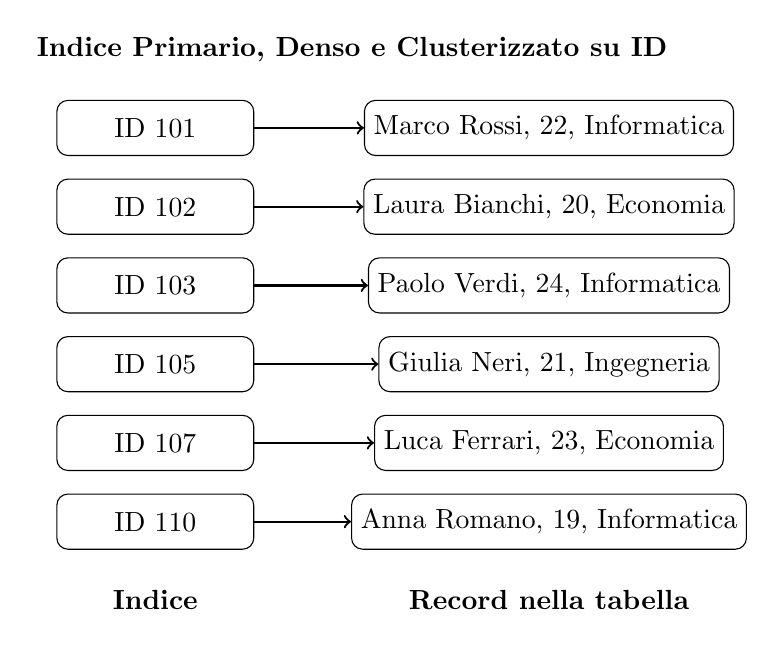
\begin{tikzpicture}[
    block/.style={rectangle, draw, rounded corners, minimum width=2.5cm, minimum height=0.7cm},
    arrow/.style={->, thick}
]
\node[block] (i1) at (0,0) {ID 101};
\node[block] (i2) at (0,-1) {ID 102};
\node[block] (i3) at (0,-2) {ID 103};
\node[block] (i4) at (0,-3) {ID 105};
\node[block] (i5) at (0,-4) {ID 107};
\node[block] (i6) at (0,-5) {ID 110};

\node[block, minimum width=4cm] (r1) at (5,0) {Marco Rossi, 22, Informatica};
\node[block, minimum width=4cm] (r2) at (5,-1) {Laura Bianchi, 20, Economia};
\node[block, minimum width=4cm] (r3) at (5,-2) {Paolo Verdi, 24, Informatica};
\node[block, minimum width=4cm] (r4) at (5,-3) {Giulia Neri, 21, Ingegneria};
\node[block, minimum width=4cm] (r5) at (5,-4) {Luca Ferrari, 23, Economia};
\node[block, minimum width=4cm] (r6) at (5,-5) {Anna Romano, 19, Informatica};

\draw[arrow] (i1) -- (r1);
\draw[arrow] (i2) -- (r2);
\draw[arrow] (i3) -- (r3);
\draw[arrow] (i4) -- (r4);
\draw[arrow] (i5) -- (r5);
\draw[arrow] (i6) -- (r6);

\node at (0,-6) {\textbf{Indice}};
\node at (5,-6) {\textbf{Record nella tabella}};
\node at (2.5,1) {\textbf{Indice Primario, Denso e Clusterizzato su ID}};
\end{tikzpicture}
\caption{Indice Primario, Denso e Clusterizzato su ID}
\end{figure}

\textbf{Caratteristiche:}
\begin{itemize}
    \item \textbf{Primario:} L'indice è sulla chiave primaria (ID) e i dati sono fisicamente ordinati per ID.
    \item \textbf{Denso:} C'è una voce nell'indice per ogni record nel file dati.
    \item \textbf{Clusterizzato:} L'ordine fisico dei dati (crescente per ID) corrisponde all'ordine dell'indice.
    \item \textbf{Vantaggi:} Ricerca efficiente per ID e per intervalli di ID (es. \texttt{ID BETWEEN 101 AND 105}).
\end{itemize}

\subsubsection{2. Indice Sparso e Clusterizzato (su ID)}

\begin{figure}[H]
\centering
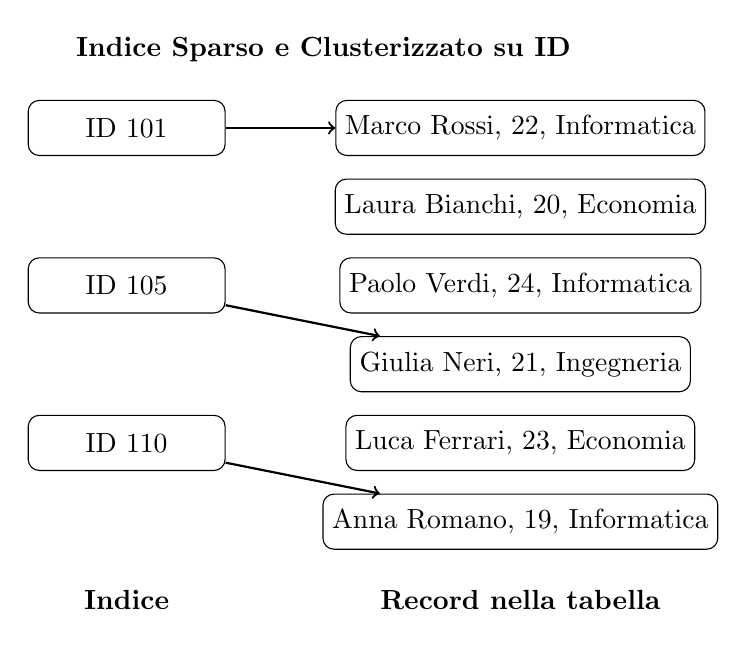
\begin{tikzpicture}[
    block/.style={rectangle, draw, rounded corners, minimum width=2.5cm, minimum height=0.7cm},
    arrow/.style={->, thick}
]
\node[block] (i1) at (0,0) {ID 101};
\node[block] (i3) at (0,-2) {ID 105};
\node[block] (i5) at (0,-4) {ID 110};

\node[block, minimum width=4cm] (r1) at (5,0) {Marco Rossi, 22, Informatica};
\node[block, minimum width=4cm] (r2) at (5,-1) {Laura Bianchi, 20, Economia};
\node[block, minimum width=4cm] (r3) at (5,-2) {Paolo Verdi, 24, Informatica};
\node[block, minimum width=4cm] (r4) at (5,-3) {Giulia Neri, 21, Ingegneria};
\node[block, minimum width=4cm] (r5) at (5,-4) {Luca Ferrari, 23, Economia};
\node[block, minimum width=4cm] (r6) at (5,-5) {Anna Romano, 19, Informatica};

\draw[arrow] (i1) -- (r1);
\draw[arrow] (i3) -- (r4);
\draw[arrow] (i5) -- (r6);

\node at (0,-6) {\textbf{Indice}};
\node at (5,-6) {\textbf{Record nella tabella}};
\node at (2.5,1) {\textbf{Indice Sparso e Clusterizzato su ID}};
\end{tikzpicture}
\caption{Indice Sparso e Clusterizzato su ID}
\end{figure}

\textbf{Caratteristiche:}
\begin{itemize}
    \item \textbf{Sparso:} Solo alcune chiavi (ogni 2-3 record in questo esempio) hanno una voce nell'indice.
    \item \textbf{Clusterizzato:} L'ordine fisico dei dati è ancora per ID crescente.
    \item \textbf{Funzionamento:} Per trovare \texttt{ID=103}, l'indice trova che \texttt{101 <= 103 < 105} e inizia la ricerca dal record con ID 101, scorrendo sequenzialmente.
    \item \textbf{Vantaggio:} Occupa meno spazio dell'indice denso, efficace quando i dati sono ordinati.
    \item \textbf{Svantaggio:} Meno efficiente nelle ricerche puntuali rispetto all'indice denso.
\end{itemize}

\subsubsection{3. Indice Secondario, Denso e Non Clusterizzato (su Facoltà)}

\begin{figure}[H]
\centering
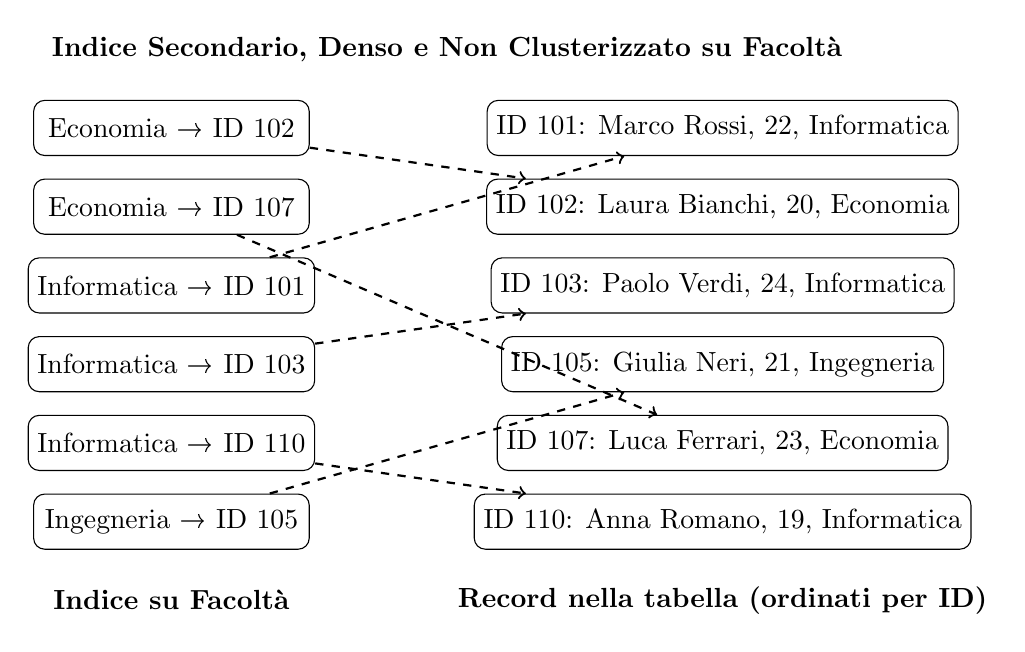
\begin{tikzpicture}[
    block/.style={rectangle, draw, rounded corners, minimum width=3.5cm, minimum height=0.7cm},
    arrow/.style={->, thick, dashed}
]
\node[block] (i1) at (0,0) {Economia → ID 102};
\node[block] (i2) at (0,-1) {Economia → ID 107};
\node[block] (i3) at (0,-2) {Informatica → ID 101};
\node[block] (i4) at (0,-3) {Informatica → ID 103};
\node[block] (i5) at (0,-4) {Informatica → ID 110};
\node[block] (i6) at (0,-5) {Ingegneria → ID 105};

\node[block, minimum width=4cm] (r1) at (7,0) {ID 101: Marco Rossi, 22, Informatica};
\node[block, minimum width=4cm] (r2) at (7,-1) {ID 102: Laura Bianchi, 20, Economia};
\node[block, minimum width=4cm] (r3) at (7,-2) {ID 103: Paolo Verdi, 24, Informatica};
\node[block, minimum width=4cm] (r4) at (7,-3) {ID 105: Giulia Neri, 21, Ingegneria};
\node[block, minimum width=4cm] (r5) at (7,-4) {ID 107: Luca Ferrari, 23, Economia};
\node[block, minimum width=4cm] (r6) at (7,-5) {ID 110: Anna Romano, 19, Informatica};

\draw[arrow] (i1) -- (r2);
\draw[arrow] (i2) -- (r5);
\draw[arrow] (i3) -- (r1);
\draw[arrow] (i4) -- (r3);
\draw[arrow] (i5) -- (r6);
\draw[arrow] (i6) -- (r4);

\node at (0,-6) {\textbf{Indice su Facoltà}};
\node at (7,-6) {\textbf{Record nella tabella (ordinati per ID)}};
\node at (3.5,1) {\textbf{Indice Secondario, Denso e Non Clusterizzato su Facoltà}};
\end{tikzpicture}
\caption{Indice Secondario, Denso e Non Clusterizzato su Facoltà}
\end{figure}

\textbf{Caratteristiche:}
\begin{itemize}
    \item \textbf{Secondario:} L'indice è su un attributo diverso dalla chiave di ordinamento dei dati (i dati sono ordinati per ID, l'indice è su Facoltà).
    \item \textbf{Denso:} C'è una voce nell'indice per ogni record nel file dati.
    \item \textbf{Non Clusterizzato:} L'ordine delle voci nell'indice (alfabetico per Facoltà) è diverso dall'ordine fisico dei dati (per ID).
    \item \textbf{Vantaggi:} Efficiente per ricerche sulla Facoltà (es. \texttt{SELECT * FROM Studenti WHERE Facoltà = 'Informatica'}).
    \item \textbf{Svantaggi:} Per trovare tutti gli studenti di Informatica, i record potrebbero essere sparsi in blocchi diversi, richiedendo più accessi al disco.
\end{itemize}

\subsubsection{Confronto dei Costi di Accesso}

\begin{table}[H]
\centering
\begin{tabular}{|p{4cm}|p{4cm}|p{4cm}|}
\hline
\textbf{Tipo di Indice} & \textbf{Costo per Ricerca Puntuale} & \textbf{Costo per Ricerca per Intervallo} \\
\hline
Denso e Clusterizzato & Basso (accesso diretto) & Molto basso (record contigui) \\
\hline
Sparso e Clusterizzato & Medio (ricerca nell'intervallo) & Basso (record contigui, ma più scansione sequenziale) \\
\hline
Secondario, Denso e Non Clusterizzato & Basso per l'attributo dell'indice, ma accessi random & Alto (record non contigui, accessi casuali a blocchi diversi) \\
\hline
\end{tabular}
\caption{Confronto dei costi di accesso per tipo di indice}
\end{table}

\textbf{Esempio di query e costo:}

\begin{minted}{sql}
-- Usando l'indice primario, denso e clusterizzato
SELECT * FROM Studenti WHERE ID = 103;  -- Accesso diretto, veloce

-- Usando l'indice sparso e clusterizzato
SELECT * FROM Studenti WHERE ID = 103;  -- Trova l'intervallo (101-105), poi scansione sequenziale dal primo record dell'intervallo. Poiché l'indice è sparso, non tutti gli ID hanno una voce nell'indice, quindi dopo aver identificato l'intervallo corretto, il DBMS deve scorrere i record in sequenza fino a trovare l'ID 103.

-- Usando l'indice secondario, denso e non clusterizzato
SELECT * FROM Studenti WHERE Facoltà = 'Informatica';  -- Trova le chiavi ma i record sono sparsi
\end{minted}

\subsection{Esercizio a Risposta Multipla}
\textbf{Domanda:} Dato un singolo file, quale affermazione è falsa?
\begin{itemize}
    \item A. Un indice denso potrebbe essere secondario.
    \item B. Un indice sparso potrebbe essere clusterizzato.
    \item C. Un indice sparso potrebbe essere non clusterizzato.
    \item D. Un indice secondario potrebbe essere clusterizzato.
\end{itemize}
\textbf{Strategia e Soluzione:}
\begin{itemize}
    \item \textbf{A. VERA.} Un indice denso su una colonna non di ordinamento dei dati è secondario.
    \item \textbf{B. VERA.} Un indice sparso richiede che i dati siano ordinati, quindi è clusterizzato.
    \item \textbf{C. FALSA.} Un indice sparso DEVE essere clusterizzato per funzionare (per poter saltare record).
    \item \textbf{D. VERA.} Puoi ordinare fisicamente la tabella secondo un indice secondario; questo lo renderebbe clusterizzato.
\end{itemize}
\textbf{Risposta corretta (la falsa): C}

\subsection{Esempio di Performance (Ricerca con Indice Denso)}
Questo esempio numerico mostra i vantaggi di un indice.
\begin{itemize}
    \item \textbf{Scenario Dati:} 1.000.000 tuple, 100.000 blocchi da 4096 byte. Spazio: 400 MB.
    \item \textbf{Scenario Indice Denso:}
    \begin{itemize}
        \item Chiave: 30 byte, Puntatore (RID): 8 byte. Coppia: 38 byte.
        \item Per blocco indice: $4096 / 38 \approx 100$ coppie (arrotondato per difetto, le slide dicono 100).
        \item Blocchi per indice: $1.000.000 / 100 = 10.000$ blocchi.
        \item Spazio per indice: $10.000 \times 4096 \text{ byte} = 40 \text{ MB}$. Può stare in memoria.
    \end{itemize}
    \item \textbf{Ricerca:} Con indice in memoria, ricerca binaria.
    \begin{itemize}
        \item Accessi per trovare chiave nell'indice: $\log_2(10.000) \approx 13-14$.
        \item Molto meglio che scansionare 100.000 blocchi di dati.
    \end{itemize}
\end{itemize}\section{Alberi B+ (B+ Trees)}
Gli alberi B+ sono una struttura dinamica comune per gli indici. Mantengono i blocchi pieni tra la metà e la totalità.

\subsection{Parametro \texorpdfstring{$n$}{n} (Ordine)}
Ogni blocco (nodo) ha spazio per:
\begin{itemize}
    \item $n$ chiavi di ricerca
    \item $n+1$ puntatori
\end{itemize}

\subsection{Esercizio: Trovare il Valore di \texorpdfstring{$n$}{n}}
\textbf{Dati:}
\begin{itemize}
    \item Dimensione Blocco: 4096 Byte
    \item Dimensione Chiave: 4 Byte
    \item Dimensione Puntatore: 8 Byte
    \item Nessun header di blocco
\end{itemize}
\textbf{Obiettivo:} Trovare il più grande intero $n$ tale che $n$ chiavi e $n+1$ puntatori stiano in un blocco.

\textbf{Formula:}
\[ (\text{Dimensione Chiave} \times n) + (\text{Dimensione Puntatore} \times (n+1)) \leq \text{Dimensione Blocco} \]
\textbf{Svolgimento:}
\[ 4n + 8(n+1) \leq 4096 \]
\[ 4n + 8n + 8 \leq 4096 \]
\[ 12n + 8 \leq 4096 \]
\[ 12n \leq 4088 \]
\[ n \leq \frac{4088}{12} \]
\[ n \leq 340.66\ldots \]
Poiché $n$ deve essere un intero, il valore massimo è $n = 340$.

\textbf{Risposta corretta: A. 340}

\subsection{Regole degli Alberi B+}
\begin{enumerate}
    \item \textbf{Nodi Foglia:}
    \begin{itemize}
        \item Contengono copie delle chiavi dal file di dati, in ordine.
        \item L'ultimo puntatore punta al \textit{prossimo nodo foglia} (lista linkata).
        \item Gli altri $n$ puntatori puntano ai \textit{record di dati effettivi} (o RID).
        \item Un nodo foglia deve essere almeno mezzo pieno (circa $\lceil (n+1)/2 \rceil$ puntatori usati, escluso il puntatore al fratello).
    \end{itemize}
    \item \textbf{Nodi Interni (Non Foglia):}
    \begin{itemize}
        \item I puntatori puntano ad altri nodi dell'albero al livello inferiore.
        \item Un nodo interno con $k$ chiavi ha $k+1$ puntatori.
        \item Se un nodo interno ha chiavi $K_1, \ldots, K_k$, il primo puntatore è per valori $< K_1$, il secondo per $\geq K_1 \text{ e } < K_2$, ecc., l'ultimo per $\geq K_k$.
        \item Un nodo interno deve avere almeno $\lceil (n+1)/2 \rceil$ puntatori usati (figli).
    \end{itemize}
    \item \textbf{Radice (Root):}
    \begin{itemize}
        \item Se non è una foglia, ha almeno due figli.
        \item Può essere meno piena della metà.
    \end{itemize}
\end{enumerate}

\subsection{Nodi Interni vs. Nodi Foglia}
Un nodo interno contiene chiavi che definiscono intervalli e puntatori ad altri nodi figli. Un nodo foglia contiene le chiavi effettive presenti nei dati e puntatori ai record corrispondenti.

\subsection{Esempio di Albero B+}
Si visualizza un albero B+ con un certo ordine $n$. La radice punta a nodi interni o foglie. I nodi interni guidano la ricerca verso i livelli inferiori in base agli intervalli di chiave. I nodi foglia contengono le chiavi finali e i puntatori ai dati, e sono collegati tra loro per scansioni di intervallo.

\begin{figure}[H]
\centering
\resizebox{\textwidth}{!}{
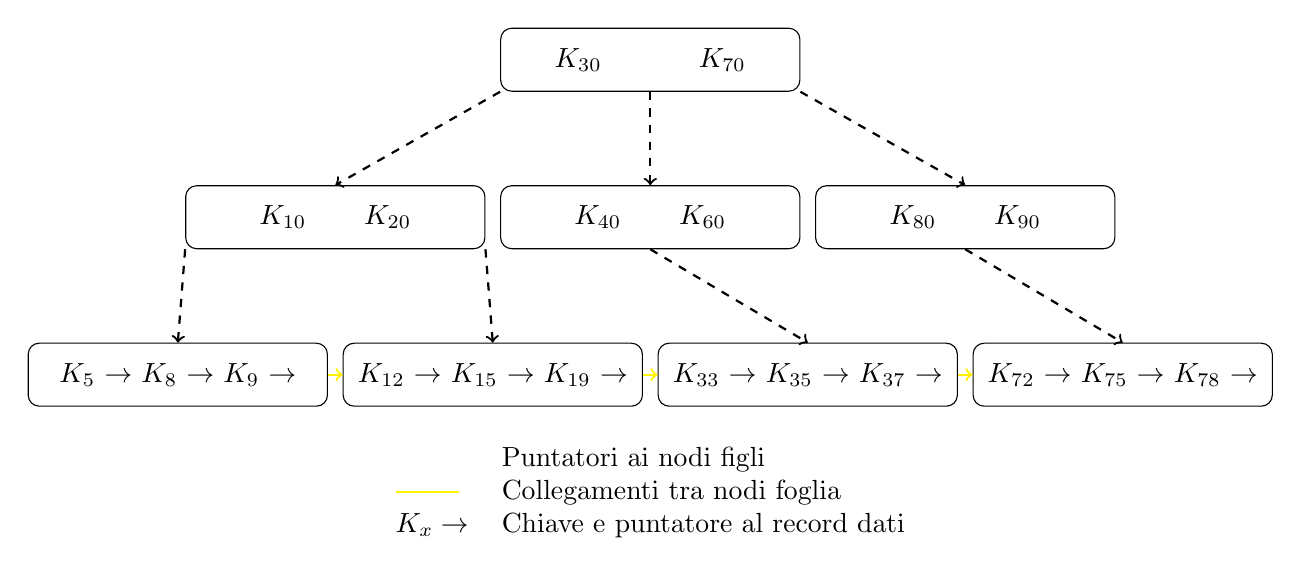
\begin{tikzpicture}[
    level distance=1.3cm,
    sibling distance=3.5cm,
    edge from parent/.style={draw, -latex},
    internal/.style={rectangle, draw, rounded corners, minimum width=3.8cm, minimum height=0.8cm, align=center},
    leaf/.style={rectangle, draw, rounded corners, minimum width=3.8cm, minimum height=0.8cm, align=center},
    pointer/.style={->, thick, dashed},
    leaf connection/.style={->, thick, yellow}
]

% Root node
\node[internal] (root) {$K_{30}$ \hspace{1cm} $K_{70}$};

% Level 1 nodes
\node[internal] (n1) at (-4,-2) {$K_{10}$ \hspace{0.5cm} $K_{20}$};
\node[internal] (n2) at (0,-2) {$K_{40}$ \hspace{0.5cm} $K_{60}$};
\node[internal] (n3) at (4,-2) {$K_{80}$ \hspace{0.5cm} $K_{90}$};

% Level 2 (leaf nodes)
\node[leaf] (l1) at (-6,-4) {$K_{5}$ $\rightarrow$ $K_{8}$ $\rightarrow$ $K_{9}$ $\rightarrow$};
\node[leaf] (l2) at (-2,-4) {$K_{12}$ $\rightarrow$ $K_{15}$ $\rightarrow$ $K_{19}$ $\rightarrow$};
\node[leaf] (l3) at (2,-4) {$K_{33}$ $\rightarrow$ $K_{35}$ $\rightarrow$ $K_{37}$ $\rightarrow$};
\node[leaf] (l4) at (6,-4) {$K_{72}$ $\rightarrow$ $K_{75}$ $\rightarrow$ $K_{78}$ $\rightarrow$};

% Connections from root to level 1
\draw[pointer] (root.south west) -- (n1.north);
\draw[pointer] (root.south) -- (n2.north);
\draw[pointer] (root.south east) -- (n3.north);

% Connections from level 1 to leaves
\draw[pointer] (n1.south west) -- (l1.north);
\draw[pointer] (n1.south east) -- (l2.north);
\draw[pointer] (n2.south) -- (l3.north);
\draw[pointer] (n3.south) -- (l4.north);

% Leaf node connections (linked list)
\draw[leaf connection] (l1.east) -- (l2.west);
\draw[leaf connection] (l2.east) -- (l3.west);
\draw[leaf connection] (l3.east) -- (l4.west);

% Legend
\node at (0,-5.5) {
\begin{tabular}{ll}
\textcolor{white}{\rule[0.5ex]{0.8cm}{1pt}} & Puntatori ai nodi figli \\
\textcolor{yellow}{\rule[0.5ex]{0.8cm}{1pt}} & Collegamenti tra nodi foglia \\
$K_x \rightarrow$ & Chiave e puntatore al record dati
\end{tabular}
};
\end{tikzpicture}
}
\caption{Struttura di un albero B+ di esempio (ordine $n=3$)}
\end{figure}

Nell'esempio, notiamo che:
\begin{itemize}
    \item I nodi interni (radice e livello intermedio) contengono chiavi che definiscono gli intervalli di ricerca.
    \item I nodi foglia contengono le chiavi effettive e i puntatori ai record di dati.
    \item I nodi foglia sono collegati tra loro (linee blu) per facilitare la scansione sequenziale.
    \item Per cercare un valore (es. $K_{35}$), seguiamo il percorso: radice $\rightarrow$ nodo intermedio $\rightarrow$ foglia appropriata.
    \item Per ricerche di intervallo (es. $K > 20$), troviamo il primo valore e poi scorriamo sequenzialmente le foglie.
\end{itemize}

\subsection{Operazioni sugli Alberi B+: Esercizi}

\subsubsection{Ricerca di Uguaglianza}
\textbf{Obiettivo:} Trovare una chiave specifica (es. K=40).
\begin{enumerate}
    \item \textbf{Radice:} Parti dalla radice. Confronta la chiave di ricerca con le chiavi nel nodo radice per determinare quale puntatore seguire.
    \item \textbf{Nodi Interni:} Continua a scendere nell'albero, seguendo il puntatore appropriato in ogni nodo interno in base all'intervallo di chiave.
    \item \textbf{Nodo Foglia:} Raggiungi un nodo foglia. Cerca la chiave di ricerca all'interno di questo nodo foglia.
    \item \textbf{Conclusione:} Se la chiave viene trovata nel nodo foglia, segui il suo puntatore per recuperare il record. Se non viene trovata, il record non esiste nell'indice.
\end{enumerate}
Descrizione del percorso di ricerca: Si parte dalla radice e si segue una traiettoria dall'alto verso il basso attraverso i nodi interni fino a raggiungere la foglia che potrebbe contenere la chiave.

\subsubsection{Ricerca per Intervallo}
\textbf{Obiettivo:} Trovare tutte le chiavi in un dato intervallo (es. K > 40).
\begin{enumerate}
    \item \textbf{Trova il primo record possibile:} Esegui una ricerca di uguaglianza per il limite inferiore dell'intervallo (es. 40). Questo ti porterà al nodo foglia che \textit{dovrebbe} contenere il primo valore dell'intervallo.
    \item \textbf{Identifica il primo valore nell'intervallo:} Esamina le chiavi nel nodo foglia trovato per identificare la prima chiave che soddisfa il criterio dell'intervallo (es. la prima chiave > 40).
    \item \textbf{Recupera i valori nell'intervallo:} Per la prima chiave trovata e per tutte le chiavi successive nel nodo foglia che sono ancora nell'intervallo, segui i puntatori associati per recuperare i record di dati.
    \item \textbf{Scorri foglie:} Se l'intervallo si estende oltre il nodo foglia corrente, segui il puntatore "prossimo nodo foglia" per spostarti al nodo foglia adiacente. Continua a elaborare le chiavi in questo nuovo nodo foglia e a spostarti ai successivi finché non esci dall'intervallo o raggiungi la fine della lista di foglie.
    \item \textbf{Risultato:} Sono stati recuperati tutti i record con chiavi nell'intervallo specificato.
\end{enumerate}
Descrizione del percorso di ricerca: Si esegue una ricerca per trovare la foglia di partenza, e poi si scorrono i nodi foglia collegati finché non si esce dall'intervallo di ricerca.

\subsubsection{Inserimento in Alberi B+}
\textbf{Principio:} Trova il nodo foglia corretto per la chiave, inserisci la chiave e il puntatore al record. Se il nodo foglia è pieno, dividilo (split) e sposta la chiave mediana (copiata) al nodo padre. Se il nodo padre è pieno, anche lui si divide e propaga una chiave al suo padre, ricorsivamente. Se la radice si divide, si crea una nuova radice e l'altezza dell'albero aumenta.

Descrizione dell'operazione di inserimento: Si individua la foglia corretta. Se c'è spazio, si inserisce. Se la foglia è piena, si divide in due, e una chiave viene copiata nel padre. Se il padre è pieno, si divide a sua volta, spostando una chiave al suo padre, e così via verso l'alto.

\subsubsection{Cancellazione da Alberi B+}
\textbf{Principio:} Trova la chiave nel nodo foglia e cancella la chiave e il puntatore al record. Se il nodo foglia scende sotto il numero minimo di chiavi/puntatori (underflow):
- Prova a \textit{prestare} una chiave dal nodo fratello adiacente che ha chiavi in eccesso. Se presti, aggiorna la chiave nel nodo padre che separa i due nodi.
- Se il fratello non può prestare, \textit{fondi} il nodo con il fratello. Durante la fusione, la chiave nel nodo padre che separava i due nodi fusi viene rimossa (se il nodo era interno) o tirata giù (se il nodo era foglia) e incorporata nel nodo fuso.
Se un nodo interno va in underflow a seguito di un prestito o fusione dei suoi figli, il processo di rebalancing (prestito/fusione) si propaga al livello superiore. Se la radice scende sotto il minimo (e non è una foglia), l'altezza dell'albero si riduce.

Descrizione dell'operazione di cancellazione: Si individua e rimuove la chiave dalla foglia. Se la foglia va in underflow, si tenta di bilanciare con un fratello (prestito o fusione). Questo può causare underflow o necessità di bilanciamento nei nodi superiori, propagandosi fino alla radice.

\subsection{Variazione dell'Altezza}
\begin{itemize}
    \item \textbf{Inserimento:} L'altezza aumenta solo se la radice corrente si divide. Una nuova radice viene creata sopra la radice divisa.
    \item \textbf{Cancellazione:} L'altezza diminuisce solo se la radice (che non è una foglia) rimane con un solo figlio a seguito di una fusione propagata, e quel figlio diventa la nuova radice.
\end{itemize}

Esempio di riduzione altezza per cancellazione: Se una fusione a livello inferiore porta la radice non-foglia ad avere un solo figlio, quel figlio diventa la nuova radice.
Esempio di aumento altezza per inserimento: Se una radice foglia piena si divide, viene creata una nuova radice interna.\section{Complessità della Ricerca con Alberi B+}
La complessità di una ricerca (uguaglianza o intervallo per trovare il primo elemento) in un albero B+ è proporzionale all'altezza $L$ dell'albero. Ogni accesso a un nodo (blocco) tipicamente richiede un accesso a disco.

Assumiamo $N_{\text{leaves}}$ è il numero totale di nodi foglia nell'albero.
Assumiamo un fattore di ramificazione (fanout) medio $m$ per i nodi interni. $m$ è approssimativamente la metà del numero massimo di puntatori ($n+1$).
L'altezza $L$ è approssimativamente data da:
\[ L \approx \log_{m}(N_{\text{leaves}}) + 1 \]
Il "+1" è per la radice.

Il numero di accessi a disco per una ricerca di uguaglianza è $L$. Per una ricerca per intervallo, è $L$ per trovare il primo elemento, più il numero di blocchi foglia da scorrere.

\subsection{Esempio di Complessità della Ricerca}
\begin{enumerate}
    \item \textbf{Calcolo di $n$ (già fatto):} Dato $n$, si sa la capacità massima dei blocchi.
    \item \textbf{Assunzioni:} Fanout medio $m$. Si stima un valore realistico per $m$ basato su $n$ e sul riempimento minimo dei nodi.
    \item \textbf{Albero B+ di $L$ livelli:} Si calcola il numero massimo (o stimato) di nodi a ogni livello e il numero totale di record indirizzabili. Con $m$ elevato, un albero B+ anche di pochi livelli può indirizzare un numero molto grande di record.
    \item \textbf{Memoria per i primi livelli:} I livelli superiori dell'albero (radice e pochi livelli sotto) sono relativamente piccoli e possono spesso risiedere nella memoria RAM del sistema di database (buffer pool).
    \item \textbf{Performance di Ricerca:} Se i livelli superiori sono in RAM, la ricerca richiede solo accessi a disco per i nodi foglia e i blocchi dati puntati. Il numero di accessi a disco è quindi ridotto e dipende dall'altezza dell'albero.
\end{enumerate}\section{Strategie Generali per gli Esercizi sugli Alberi B+}
\begin{enumerate}
    \item \textbf{Capire $n$:} Calcola o ti viene dato il valore di $n$ e i requisiti minimi per i nodi.
    \item \textbf{Distinguere Nodi Interni e Foglie:} Ricorda la loro struttura e funzione differente.
    \item \textbf{Ricerca:} Applica la ricerca dall'alto verso il basso per trovare la foglia o il punto di partenza per un intervallo.
    \item \textbf{Inserimento:} Individua la foglia. Inserisci. Gestisci gli split e la propagazione verso l'alto. Considera l'aumento dell'altezza.
    \item \textbf{Cancellazione:} Individua la chiave nella foglia. Cancella. Gestisci l'underflow con prestito o fusione. Propaga il rebalancing verso l'alto. Considera la riduzione dell'altezza.
    \item \textbf{Disegna l'albero:} Per esercizi che richiedono di mostrare lo stato dell'albero, disegnare l'albero passo passo è cruciale.
\end{enumerate}

